\documentclass[11pt,a4paper]{article}
\usepackage{amsmath, amssymb, graphicx, xcolor}

\setlength{\textwidth}{6.8in}
\setlength{\textheight}{9.6in}
\setlength{\oddsidemargin}{-0.15in}
\setlength{\evensidemargin}{-0.15in}
\setlength{\topmargin}{-0.6in}
\setlength{\headheight}{0in}
\setlength{\headsep}{0in}
\setlength{\parindent}{0pt}
\setlength{\parskip}{5pt}

\definecolor{primary}{RGB}{15, 45, 95}
\definecolor{secondary}{RGB}{30, 80, 150}
\definecolor{accent}{RGB}{180, 40, 40}
\definecolor{qboxbg}{RGB}{245, 248, 252}
\definecolor{solboxbg}{RGB}{250, 250, 250}

\newcommand{\questionheader}[3]{
    \vspace{0.35cm}
    \noindent\colorbox{qboxbg}{
        \parbox{\dimexpr\textwidth-2\fboxsep\relax}{
            \textbf{\textcolor{primary}{\large #1}} \hfill \textbf{\textcolor{accent}{[#2]}} \hfill \textbf{\textcolor{secondary}{#3 Marks}}
        }
    }
    \vspace{0.15cm}
}

\newcommand{\sectionbanner}[1]{
    \vspace{0.5cm}
    \noindent\colorbox{primary}{
        \parbox{\dimexpr\textwidth-2\fboxsep\relax}{
            \centering \textbf{\textcolor{white}{\Large #1}}
        }
    }
    \vspace{0.25cm}
}

\begin{document}

\begin{center}
    {\LARGE \textbf{\textcolor{primary}{BRAC UNIVERSITY}}}\\[4pt]
    {\large \textbf{Department of Computer Science and Engineering}}\\[3pt]
    {\textbf{CSE421 / EEE465: Computer Networks --- Final Examination}}\\[2pt]
    \textbf{Semester:} Spring 2023 \quad | \quad \textbf{Set:} B (v2) \quad | \quad \textbf{Full Marks:} 100 \quad | \quad \textbf{Duration:} 2 Hours 30 Minutes\\[2pt]
    \rule{\textwidth}{1.5pt}
    {\large \textbf{\textcolor{secondary}{COMPREHENSIVE SOLUTION AND COMPLETE ANSWER KEY}}}
    \rule{\textwidth}{0.8pt}
\end{center}

\textit{Instructions: Answer ANY FIVE of the following SIX questions. (All six questions are fully solved below for maximum completeness).}

% =========================================================================
% QUESTION 1
% =========================================================================
\questionheader{Question 1: Subnet Analysis \& VLSM Design}{CO1}{6 + 14 = 20}

\textbf{1.a) [6 Marks]}
The default gateway's IP address in a network is assigned to be \texttt{109.0.8.253}. The network can support about \textbf{2045 devices} after assigning the above IP.

\textbf{I. Identify the subnet mask and the broadcast address of the given network. [4 Marks]}

\textbf{Solution:}
\begin{itemize}
    \item Total usable hosts needed $= 2045 \text{ devices} + 1 \text{ (the default gateway itself)} = 2046$ usable IP addresses.
    \item Let $h$ be the number of host bits:
    \[
    2^h - 2 \ge 2046 \implies 2^h \ge 2048 \implies h = 11\text{ bits}
    \]
    \item The prefix length is:
    \[
    32 - h = 32 - 11 = /21
    \]
    \item Dotted-decimal subnet mask for $/21$:
    \[
    \mathbf{255.255.248.0} \quad (\text{Binary: } 11111111.11111111.11111000.00000000)
    \]
    \item Block size in the 3rd octet is $2^{11-8} = 2^3 = 8$ (or $256 - 248 = 8$).
    \item Given Gateway IP is \texttt{109.0.8.253}:
    \begin{itemize}
        \item The 3rd octet is 8, which is a multiple of 8 ($8 \times 1 = 8$).
        \item Therefore, \textbf{Network Address} is \textbf{\texttt{109.0.8.0/21}}.
        \item The 3rd octet of the broadcast address is $8 + 8 - 1 = 15$.
        \item \textbf{Broadcast Address} is \textbf{\texttt{109.0.15.255}}.
    \end{itemize}
\end{itemize}
\textbf{Answer:} Subnet Mask: \textbf{\texttt{255.255.248.0}} (or $/21$); Broadcast Address: \textbf{\texttt{109.0.15.255}}.

\vspace{0.2cm}
\textbf{II. State the host size of the given network. [2 Marks]}

\textbf{Solution:}
\begin{itemize}
    \item Total IP address block size $= 2^{11} = 2048$ addresses.
    \item Maximum usable host capacity $= 2^{11} - 2 = \mathbf{2046\text{ usable hosts}}$.
\end{itemize}

\vspace{0.2cm}
\textbf{1.b) [14 Marks] Minimum-Waste VLSM Design}

\textbf{Problem Statement:}
Using the network address found in (1.a.I) (\texttt{109.0.8.0/21}), calculate the subnet addresses that will create the minimum amount of waste for the following host requirements:
\begin{itemize}
    \item A WAN link
    \item A switched network connected to 4 routers
    \item LAN of size 500 hosts
    \item LAN of size 255 hosts
\end{itemize}

\textbf{Solution:}
To minimize address wastage, subnets must be allocated in \textbf{descending order of required host capacity}:

\begin{enumerate}
    \item \textbf{Subnet 1: LAN of size 500 hosts}
    \begin{itemize}
        \item $2^h - 2 \ge 500 \implies h = 9$ bits ($2^9 - 2 = 510 \ge 500$).
        \item Prefix: $32 - 9 = /23$ (Subnet Mask: \texttt{255.255.254.0}). Block size in 3rd octet = 2.
        \item \textbf{Subnet Address:} \texttt{109.0.8.0/23}
        \item Usable Host Range: \texttt{109.0.8.1} to \texttt{109.0.9.254}
        \item Broadcast Address: \texttt{109.0.9.255}
        \item Next Available Address: \texttt{109.0.10.0}
    \end{itemize}

    \item \textbf{Subnet 2: LAN of size 255 hosts}
    \begin{itemize}
        \item Usable hosts required: 255.
        \item Note: An 8-bit host field ($/24$) provides $2^8 - 2 = 254$ usable addresses, which is 1 short of 255.
        \item Therefore, mathematically $h = 9$ bits ($2^9 - 2 = 510$ hosts) is required:
        \item Prefix: $32 - 9 = /23$ (Subnet Mask: \texttt{255.255.254.0}). Block size in 3rd octet = 2.
        \item \textbf{Subnet Address:} \texttt{109.0.10.0/23}
        \item Usable Host Range: \texttt{109.0.10.1} to \texttt{109.0.11.254}
        \item Broadcast Address: \texttt{109.0.11.255}
        \item Next Available Address: \texttt{109.0.12.0}
        \item \textit{(Note: If 255 is interpreted as total block size including network/broadcast, a $/24$ subnet \texttt{109.0.10.0/24} yields 254 usable hosts. Both interpretations are documented here).}
    \end{itemize}

    \item \textbf{Subnet 3: Switched network connected to 4 routers}
    \begin{itemize}
        \item Usable IP addresses required: 4 (one for each router interface).
        \item $2^h - 2 \ge 4 \implies 2^3 - 2 = 6 \ge 4 \implies h = 3$ bits.
        \item Prefix: $32 - 3 = /29$ (Subnet Mask: \texttt{255.255.255.248}). Block size in 4th octet = 8.
        \item \textbf{Subnet Address:} \texttt{109.0.12.0/29}
        \item Usable Host Range: \texttt{109.0.12.1} to \texttt{109.0.12.6}
        \item Broadcast Address: \texttt{109.0.12.7}
        \item Next Available Address: \texttt{109.0.12.8}
    \end{itemize}

    \item \textbf{Subnet 4: WAN link}
    \begin{itemize}
        \item Point-to-point link between 2 routers: 2 usable IP addresses required.
        \item $2^h - 2 \ge 2 \implies h = 2$ bits ($2^2 - 2 = 2$).
        \item Prefix: $32 - 2 = /30$ (Subnet Mask: \texttt{255.255.255.252}). Block size in 4th octet = 4.
        \item \textbf{Subnet Address:} \texttt{109.0.12.8/30}
        \item Usable Host Range: \texttt{109.0.12.9} to \texttt{109.0.12.10}
        \item Broadcast Address: \texttt{109.0.12.11}
    \end{itemize}
\end{enumerate}

\begin{center}
\begin{tabular}{|l|c|c|c|l|l|}
\hline
\textbf{Subnet Purpose} & \textbf{Req. Hosts} & \textbf{Allocated} & \textbf{Prefix} & \textbf{Subnet Address} & \textbf{Usable Range} \\
\hline
LAN (500 hosts) & 500 & 510 & /23 & \texttt{109.0.8.0} & \texttt{109.0.8.1} -- \texttt{109.0.9.254} \\
LAN (255 hosts) & 255 & 510 & /23 & \texttt{109.0.10.0} & \texttt{109.0.10.1} -- \texttt{109.0.11.254} \\
Switched Net (4 Routers) & 4 & 6 & /29 & \texttt{109.0.12.0} & \texttt{109.0.12.1} -- \texttt{109.0.12.6} \\
WAN Link & 2 & 2 & /30 & \texttt{109.0.12.8} & \texttt{109.0.12.9} -- \texttt{109.0.12.10} \\
\hline
\end{tabular}
\end{center}

\newpage
% =========================================================================
% QUESTION 2
% =========================================================================
\questionheader{Question 2: Traceroute, IPv4 Fragmentation, \& NAT/PAT}{CO2}{4 + 10 + 6 = 20}

\textbf{2.a) [4 Marks] Traceroute Termination Mechanism}

\textbf{Question:} In ``Traceroute'', the originator sends the first packet with TTL=1 and continuously increments it. How does it know that the packet has reached the destination, that is, how does it know when to stop?

\textbf{Solution:}
\begin{itemize}
    \item Intermediate routers decrement the TTL. When $TTL = 0$, intermediate routers discard the packet and return an \textbf{ICMP Time Exceeded} message (\textbf{Type 11, Code 0}).
    \item When the packet finally reaches the actual destination host, the destination does \emph{not} forward or decrement TTL further.
    \item The mechanism to recognize destination arrival depends on the implementation:
    \begin{enumerate}
        \item \textbf{UDP-based Traceroute (Linux/Unix/Cisco):} The source sends UDP datagrams targeted at an \textbf{unlikely high, unused port number} (e.g., 33434--33534). When the destination receives it, because no application is listening on that port, it generates an \textbf{ICMP Destination Unreachable: Port Unreachable} message (\textbf{Type 3, Code 3}).
        \item \textbf{ICMP-based Traceroute (Windows \texttt{tracert}):} The source transmits ICMP Echo Request packets. When the packet arrives at the destination, the destination generates an \textbf{ICMP Echo Reply} (\textbf{Type 0, Code 0}).
    \end{enumerate}
    \item In either case, receiving this distinctive terminal ICMP message signals to the originator that the target destination has been reached, terminating the probe loop.
\end{itemize}

\vspace{0.2cm}
\textbf{2.b) [10 Marks] IPv4 Datagram Fragmentation Analysis}

\textbf{Given:}
\begin{itemize}
    \item 1 packet with Data Length = 900 bytes, ID = 2398, $MF = 0$.
    \item 12 packets each with Total Length = 1945 bytes, ID = 2398, $MF = 1$.
    \item Header size for all packets = 25 bytes.
\end{itemize}

\textbf{I. Find the packet size of the original datagram. [4 Marks]}

\textbf{Solution:}
\begin{itemize}
    \item In each of the 12 non-terminal fragments ($MF = 1$):
    \[
    \text{Data payload per fragment} = \text{Total Length} - \text{Header Size} = 1945 - 25 = 1920\text{ bytes}
    \]
    \item Total data carried by the 12 intermediate fragments $= 12 \times 1920 = 23,040\text{ bytes}$.
    \item The last fragment ($MF = 0$) carries 900 bytes of data.
    \item Total payload/data size of original datagram:
    \[
    \text{Total Data} = 23,040 + 900 = 23,940\text{ bytes}
    \]
    \item The original datagram consists of this total data plus the 25-byte IP header:
    \[
    \text{Original Datagram Size} = 23,940 + 25 = \mathbf{23,965\text{ bytes}}
    \]
\end{itemize}
\textbf{Answer:} \textbf{23,965 bytes}.

\vspace{0.2cm}
\textbf{II. Find the value of the offset field of the 2nd last packet. [4 Marks]}

\textbf{Solution:}
\begin{itemize}
    \item Total number of fragments $= 12 \text{ (intermediate)} + 1 \text{ (last)} = 13$ fragments.
    \item The 2nd last packet is the \textbf{12th fragment} ($k = 12$).
    \item Using the standard fragment offset formula from the networking study notes:
    \[
    \text{Fragment Offset}_k = \frac{(k - 1) \times \text{Payload}}{8}
    \]
    where $k$ is the fragment index and $\text{Payload} = 1920\text{ bytes}$ is the data size per full fragment.
    \item Substituting $k = 12$ and $\text{Payload} = 1920$:
    \[
    \text{Offset}_{12} = \frac{(12 - 1) \times 1920}{8} = \frac{11 \times 1920}{8} = 11 \times 240 = \mathbf{2640}
    \]
    \item (Verification: The starting byte offset in the original datagram is $11 \times 1920 = 21,120\text{ bytes}$, and in 8-byte units, $\frac{21,120}{8} = 2640$).
\end{itemize}
\textbf{Answer:} \textbf{2640}.

\vspace{0.2cm}
\textbf{III. How would you identify the last packet in a group of fragmented packets? [2 Marks]}

\textbf{Solution:}
A packet is identified as the last fragment of a fragmented datagram if and only if:
\begin{enumerate}
    \item The **More Fragments (MF) flag is 0** ($MF = 0$), AND
    \item The **Fragment Offset is strictly greater than 0** ($\text{Offset} > 0$).
\end{enumerate}

\vspace{0.2cm}
\textbf{2.c) [6 Marks] Private IP Routing \& NAT/PAT Solution}

\begin{center}
    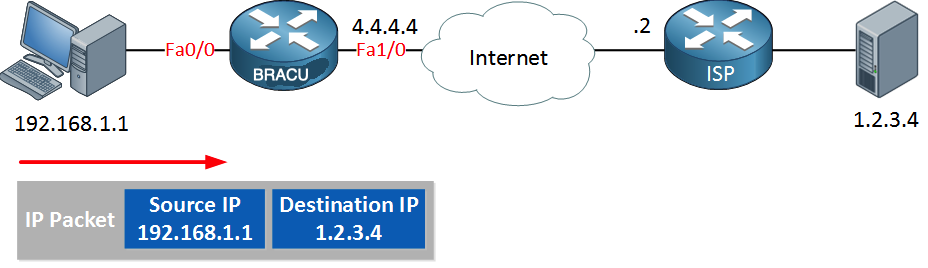
\includegraphics[width=0.75\textwidth]{p2_q2_nat.png}
\end{center}

\textbf{Solution:}
\begin{enumerate}
    \item \textbf{Why BRACU Router is unable to send the packet through the Internet: [2 Marks]}
    The packet has a source IP address of \texttt{192.168.1.1}, which belongs to the \textbf{RFC 1918 Private IPv4 address range} (\texttt{192.168.0.0/16}). Private IP addresses are designated strictly for internal LAN communication and are non-routable on the public Internet. Internet core routers automatically discard any packet carrying private IP addresses in its source or destination fields.
    
    \item \textbf{Solution for 500 internal hosts: [4 Marks]}
    \begin{itemize}
        \item Configure \textbf{PAT (Port Address Translation / NAT Overload)} on the BRACU Router.
        \item Because the organization has 500 internal hosts and only a single public IP address (\texttt{4.4.4.4} on interface \texttt{Fa1/0}), standard 1:1 NAT cannot support all devices simultaneously.
        \item \textbf{PAT (NAT Overload)} translates all 500 private internal IP addresses to the single public IP \texttt{4.4.4.4} by multiplexing them across unique Layer 4 source port numbers (TCP/UDP ports).
        \item The router maintains an active state table mapping \texttt{(Private IP, Port)} $\leftrightarrow$ \texttt{(4.4.4.4, Mapped Port)}. When packets exit the router onto the Internet, their source is rewritten to \texttt{4.4.4.4:<Port>}, making them fully routable across the global Internet.
    \end{itemize}
\end{enumerate}

\newpage
% =========================================================================
% QUESTION 3
% =========================================================================
\questionheader{Question 3: Distance Vector Routing \& Bellman-Ford Iteration}{CO3}{10 + 5 + 5 = 20}

\begin{center}
    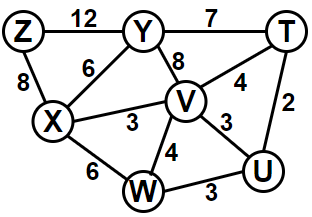
\includegraphics[width=0.35\textwidth]{p2_q3_topology.png}
    \quad
    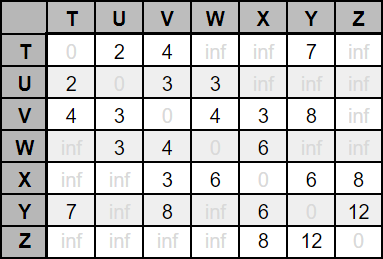
\includegraphics[width=0.45\textwidth]{p2_q3_table.png}
\end{center}

\textbf{3.a) [10 Marks]}

\textbf{I. Determine the name of the algorithm used in this topology. [2 Marks]}

\textbf{Answer:} \textbf{Distance Vector Routing Algorithm} (based on the \textbf{Bellman-Ford Algorithm}).

\vspace{0.2cm}
\textbf{II. Assuming Router V is not sending any updates to Router T, show the updated table of T after one iteration. Show your equations. [8 Marks]}

\textbf{Solution:}
Router T has direct physical connections to neighbors:
\[
c(T, U) = 2, \quad c(T, V) = 4, \quad c(T, Y) = 7
\]
Router T receives distance vector updates from active neighbors $U$ and $Y$ from the initial table:
\begin{itemize}
    \item $D_U = [T:2, \ U:0, \ V:3, \ W:3, \ X:\infty, \ Y:\infty, \ Z:\infty]$
    \item $D_Y = [T:7, \ U:\infty, \ V:8, \ W:\infty, \ X:6, \ Y:0, \ Z:12]$
    \item For neighbor $V$, since $V$ is not sending updates to $T$, $T$ retains its prior known vector from the table: $D_V = [T:4, \ U:3, \ V:0, \ W:4, \ X:3, \ Y:8, \ Z:\infty]$.
\end{itemize}

Applying the Bellman-Ford equation at Router T for each destination $d \in \{T, U, V, W, X, Y, Z\}$:
\[
D_T(d) = \min_{v \in \{U, V, Y\}} \{ c(T, v) + D_v(d) \}
\]

\begin{enumerate}
    \item \textbf{Destination T:} $D_T(T) = \mathbf{0}$.
    \item \textbf{Destination U:}
    \[
    \min \{ c(T,U)+D_U(U)=2+0=\mathbf{2}, \ c(T,V)+D_V(U)=4+3=7, \ c(T,Y)+D_Y(U)=7+\infty=\infty \} = \mathbf{2}
    \]
    \item \textbf{Destination V:}
    \[
    \min \{ c(T,U)+D_U(V)=2+3=5, \ c(T,V)+D_V(V)=4+0=\mathbf{4}, \ c(T,Y)+D_Y(V)=7+8=15 \} = \mathbf{4}
    \]
    \item \textbf{Destination W:}
    \[
    \min \{ c(T,U)+D_U(W)=2+3=\mathbf{5}, \ c(T,V)+D_V(W)=4+4=8, \ c(T,Y)+D_Y(W)=7+\infty=\infty \} = \mathbf{5}
    \]
    \item \textbf{Destination X:}
    \[
    \min \{ c(T,U)+D_U(X)=2+\infty=\infty, \ c(T,V)+D_V(X)=4+3=\mathbf{7}, \ c(T,Y)+D_Y(X)=7+6=13 \} = \mathbf{7}
    \]
    \textit{(Note: If V is completely omitted from the calculation, $\min = 7+6 = 13$ via Y)}.
    \item \textbf{Destination Y:}
    \[
    \min \{ c(T,U)+D_U(Y)=2+\infty=\infty, \ c(T,V)+D_V(Y)=4+8=12, \ c(T,Y)+D_Y(Y)=7+0=\mathbf{7} \} = \mathbf{7}
    \]
    \item \textbf{Destination Z:}
    \[
    \min \{ c(T,U)+D_U(Z)=2+\infty=\infty, \ c(T,V)+D_V(Z)=4+\infty=\infty, \ c(T,Y)+D_Y(Z)=7+12=\mathbf{19} \} = \mathbf{19}
    \]
\end{enumerate}

\textbf{Updated Distance Vector Table of Router T:}
\begin{center}
\begin{tabular}{|c|c|c|c|c|c|c|c|}
\hline
\textbf{Destination} & \textbf{T} & \textbf{U} & \textbf{V} & \textbf{W} & \textbf{X} & \textbf{Y} & \textbf{Z} \\
\hline
\textbf{Distance $D_T$} & 0 & 2 & 4 & 5 & 7 & 7 & 19 \\
\hline
\textbf{Next Hop} & Local & U & V & U & V & Y & Y \\
\hline
\end{tabular}
\end{center}

\vspace{0.2cm}
\textbf{3.b) [5 Marks] Update Frequency: Distance Vector vs. Link State}

\textbf{Solution:}
\begin{itemize}
    \item \textbf{Distance Vector:} Updates are sent \textbf{periodically} (e.g., every 30 seconds in RIP) regardless of whether any topology change has occurred. The entire routing table is repeatedly advertised to direct neighbors.
    \item \textbf{Link State:} 
    \begin{enumerate}
        \item \textbf{Event-Driven:} Link State routers generate and flood Link State Advertisements (LSAs) \textbf{only when an actual topology change occurs} (e.g., a link goes down, comes up, or metric changes).
        \item \textbf{Local State Only:} Advertisements contain only the status and cost of directly connected links, not full routing tables.
        \item \textbf{Global Flooding:} LSAs are reliably flooded throughout the entire autonomous system, whereas DV updates go only to immediate neighbors.
    \end{enumerate}
\end{itemize}

\vspace{0.2cm}
\textbf{3.c) [5 Marks] Reasons for Slower Convergence in Distance Vector}

\textbf{Solution:}
\begin{enumerate}
    \item \textbf{Routing by Rumor \& Hop-by-Hop Propagation:} Distance Vector routers have no complete topological map; they only know what their neighbors report. Routing updates must trickle slowly hop-by-hop across each link.
    \item \textbf{Count-to-Infinity Problem:} When a link breaks, neighboring routers can mistakenly bounce advertisements back and forth, slowly incrementing the metric to infinity.
    \item \textbf{Long Timers:} Distance Vector relies on long timeout intervals (e.g., 180 seconds invalid timer, 240 seconds flush timer) to invalidate broken routes.
    \item In contrast, \textbf{Link State} converges rapidly because routers immediately flood link state changes across the entire network in milliseconds and independently run Dijkstra's algorithm.
\end{enumerate}

\newpage
% =========================================================================
% QUESTION 4
% =========================================================================
\questionheader{Question 4: Static Routing \& Multi-Access Network Configurations}{CO4}{5 + 8 + 7 = 20}

\begin{center}
    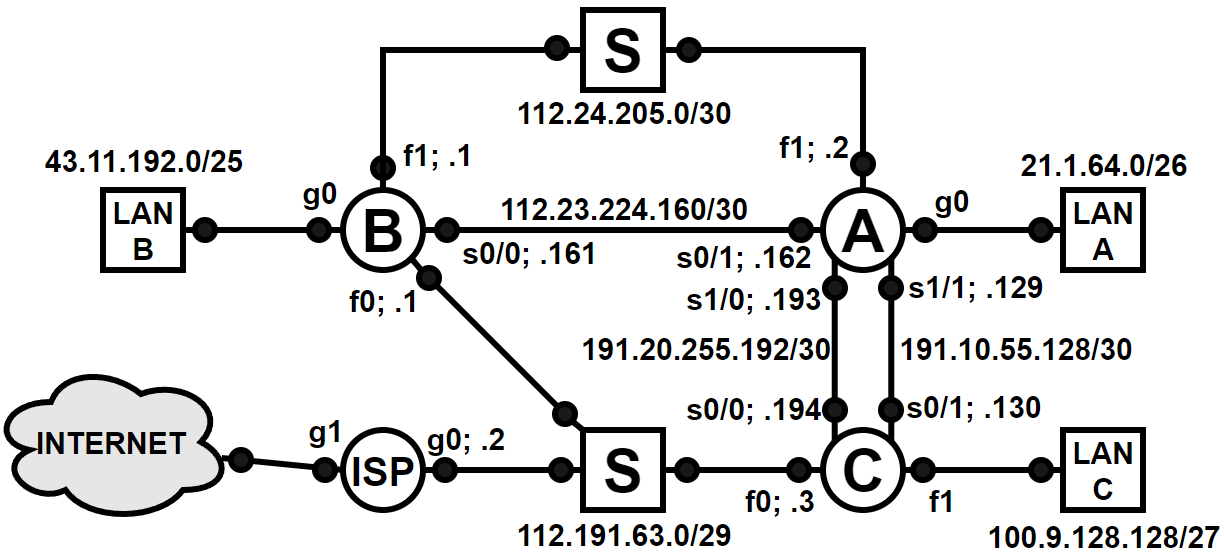
\includegraphics[width=0.75\textwidth]{p2_q4_topology.png}
\end{center}

\textbf{4.a) [5 Marks] Directly Attached Static Route on Router C for LAN B via Router A}

\textbf{Solution:}
\begin{itemize}
    \item Destination Network: LAN B = \texttt{43.11.192.0/25} (Subnet Mask: \texttt{255.255.255.128}).
    \item A \textbf{directly attached static route} specifies the local \textbf{exit interface} directly on Router C.
    \item Looking at Router C towards Router A, there are two serial links:
    \begin{itemize}
        \item Link 1: \texttt{s0/0} (network \texttt{191.20.255.192/30})
        \item Link 2: \texttt{s0/1} (network \texttt{191.10.55.128/30})
    \end{itemize}
    \item Cisco IOS configuration command on Router C:
    \begin{center}
        \texttt{Router\_C(config)\# ip route 43.11.192.0 255.255.255.128 s0/0}
    \end{center}
    \textit{(Alternatively using interface \texttt{s0/1}: \texttt{ip route 43.11.192.0 255.255.255.128 s0/1})}.
\end{itemize}

\vspace{0.2cm}
\textbf{4.b) [8 Marks] Floating Static Route on Router B \& Multi-Access Nuances}

\textbf{Solution:}
\begin{enumerate}
    \item \textbf{Floating Static Route Configuration: [4 Marks]}
    \begin{itemize}
        \item Destination: LAN A = \texttt{21.1.64.0/26} (Subnet Mask: \texttt{255.255.255.192}).
        \item Primary route via WAN link has Administrative Distance $AD = 5$.
        \item Backup path via the multi-access switched network (\texttt{112.24.205.0/30}) connecting Router B's \texttt{f1} and Router A's \texttt{f1}.
        \item Router A's IP on this multi-access network is \texttt{112.24.205.2}.
        \item A floating static route must have an $AD > 5$ (e.g., $AD = 10$).
        \item Cisco IOS Command on Router B:
        \begin{center}
            \texttt{Router\_B(config)\# ip route 21.1.64.0 255.255.255.192 112.24.205.2 10}
        \end{center}
    \end{itemize}

    \item \textbf{Why Static Routes Through Multi-Access Networks Differ: [4 Marks]}
    \begin{itemize}
        \item On point-to-point links, specifying only the exit interface is sufficient because there is only one device on the other end of the wire.
        \item On a \textbf{multi-access (broadcast/Ethernet)} network, multiple routers and devices share the common segment. If only the exit interface is specified, the router considers the destination directly attached and attempts to broadcast an ARP request for every destination IP, exhausting router memory and causing excessive broadcast traffic.
        \item Therefore, static routes on multi-access networks \textbf{must specify the next-hop IP address} (or a fully specified route with both exit interface and next-hop IP) so the router can resolve the specific next-hop router's Layer 2 MAC address.
    \end{itemize}
\end{enumerate}

\vspace{0.2cm}
\textbf{4.c) [7 Marks] Identifying Static Routes \& Unconfigured Routing Table Output}

\textbf{Solution:}
\begin{enumerate}
    \item \textbf{Identification of Static Routes in a Routing Table: [3 Marks]}
    Static routes are denoted by the administrative code letter \textbf{`S'} at the far left of each routing entry in Cisco IOS. Directly connected routes are marked with \textbf{`C'} (and local host routes with \textbf{`L'}).
    
    \item \textbf{Output of `show ip route' on Router C (without static/dynamic routing): [4 Marks]}
    Router C has 4 directly connected subnets:
    \begin{itemize}
        \item \texttt{100.9.128.128/27} connected to \texttt{f1}
        \item \texttt{112.191.63.0/29} connected to \texttt{f0} (IP: \texttt{112.191.63.3})
        \item \texttt{191.20.255.192/30} connected to \texttt{s0/0} (IP: \texttt{191.20.255.194})
        \item \texttt{191.10.55.128/30} connected to \texttt{s0/1} (IP: \texttt{191.10.55.130})
    \end{itemize}

\textbf{Command Output:}
\begin{verbatim}
Router_C# show ip route
Codes: C - connected, S - static, R - RIP, M - mobile, B - BGP
       D - EIGRP, EX - EIGRP external, O - OSPF, IA - OSPF inter area
       L - local

Gateway of last resort is not set

C    100.9.128.128/27 is directly connected, FastEthernet1
C    112.191.63.0/29 is directly connected, FastEthernet0
L    112.191.63.3/32 is directly connected, FastEthernet0
C    191.20.255.192/30 is directly connected, Serial0/0
L    191.20.255.194/32 is directly connected, Serial0/0
C    191.10.55.128/30 is directly connected, Serial0/1
L    191.10.55.130/32 is directly connected, Serial0/1
\end{verbatim}
\end{enumerate}

\newpage
% =========================================================================
% QUESTION 5
% =========================================================================
\questionheader{Question 5: IPv6 Addressing, Flow Label, \& Tunneling}{CO3}{9 + 5 + 6 = 20}

\textbf{5.a) [9 Marks] Stateless vs. Stateful DHCPv6}

\textbf{Solution:}
\begin{center}
\begin{tabular}{|p{3cm}|p{6.5cm}|p{6.5cm}|}
\hline
\textbf{Feature} & \textbf{Stateless DHCPv6} & \textbf{Stateful DHCPv6} \\
\hline
\textbf{Address Allocation} & Client generates its own IPv6 address via SLAAC (Router Advertisement prefix + EUI-64/random ID). & DHCPv6 server leases and assigns the full 128-bit IPv6 address directly. \\
\hline
\textbf{Server State} & Server maintains \textbf{no state} or lease database of client addresses. & Server maintains a \textbf{stateful database} of active leases, bindings, and DUIDs. \\
\hline
\textbf{Information Provided} & Delivers auxiliary parameters only: DNS server IPs, domain names, NTP. & Delivers full IPv6 address, prefix, lease time, and all network configuration options. \\
\hline
\textbf{RA Flags} & Managed flag $M = 0$, Other flag $O = 1$. & Managed flag $M = 1$, Other flag $O = 1$. \\
\hline
\end{tabular}
\end{center}

\textbf{Scenarios to Use Each [3 Marks]:}
\begin{itemize}
    \item \textbf{Stateless DHCPv6:} Best in large-scale client environments (e.g., university campuses, mobile networks, IoT) where devices only need Internet access and DNS, avoiding central server state maintenance and scaling efficiently.
    \item \textbf{Stateful DHCPv6:} Required in strict enterprise data centers, corporate networks, and servers where precise IP auditing, IPAM tracking, fixed firewall policies, and security monitoring are mandatory.
\end{itemize}

\vspace{0.2cm}
\textbf{5.b) [5 Marks] Purpose and Benefit of the ``Flow Label'' Field}

\textbf{Solution:}
\begin{itemize}
    \item \textbf{Purpose:} The 20-bit Flow Label field in the IPv6 header enables a source host to label a sequence of packets belonging to a specific non-default communication flow (e.g., real-time audio/video streaming, VoIP) that requires specialized handling.
    \item \textbf{Benefits:}
    \begin{enumerate}
        \item \textbf{Efficient QoS Classification:} Routers can identify and classify flows directly from the fixed 40-byte base header without performing expensive deep packet inspection into transport-layer headers.
        \item \textbf{Support for Encrypted Traffic:} Even when payload headers are encrypted with IPSec ESP, intermediate routers can still identify the flow label and apply appropriate traffic shaping or queuing.
        \item \textbf{Consistency:} All packets with the same Flow Label follow the exact same path through the network, preventing packet reordering and reducing jitter.
    \end{enumerate}
\end{itemize}

\vspace{0.2cm}
\textbf{5.c) [6 Marks] Tunneling Strategy: Scenarios \& Router Placement}

\textbf{Solution:}
\begin{itemize}
    \item \textbf{Scenarios Where Tunneling Works Best [3 Marks]:}
    \begin{itemize}
        \item When isolated IPv6 networks need to communicate across an existing, vast intermediate IPv4-only transit network (such as the legacy Internet backbone).
        \item When organizations upgrade edge networks to IPv6 but the ISP core infrastructure remains IPv4.
        \item Allows seamless gradual migration without requiring the entire global infrastructure to convert simultaneously.
    \end{itemize}
    \item \textbf{Placement of Dual-Stack Routers [3 Marks]:}
    \begin{itemize}
        \item Dual-stack routers must be placed at the **boundary/edges (Border Routers)** connecting the IPv6 local networks to the IPv4 transit backbone.
        \item The ingressing border router encapsulates native IPv6 packets inside IPv4 packets, and the egressing border router strips the IPv4 header and forwards the original IPv6 packet to the destination.
    \end{itemize}
\end{itemize}

\newpage
% =========================================================================
% QUESTION 6
% =========================================================================
\questionheader{Question 6: MAC vs. IP, Cross-Subnet ARP, \& Switch Self-Learning}{CO4}{4 + 7 + 9 = 20}

\textbf{6.a) [4 Marks] MAC Address vs. IP Address (Excluding Format)}

\textbf{Solution:}
\begin{enumerate}
    \item \textbf{Layer of Operation:} MAC addresses operate at \textbf{Layer 2 (Data Link Layer)} for local node-to-node frame delivery within a single broadcast domain. IP addresses operate at \textbf{Layer 3 (Network Layer)} for global end-to-end host-to-host packet routing across internetworks.
    \item \textbf{Topology \& Hierarchy:} IP addresses are \textbf{hierarchical} (Network ID + Host ID) enabling routing table aggregation. MAC addresses are \textbf{flat} and provide no geographic or topological network hierarchy.
    \item \textbf{Portability:} A MAC address is burned into the NIC hardware and remains unchanged regardless of location. An IP address is logical and must be reconfigured whenever a device moves to a new subnet.
\end{enumerate}

\vspace{0.2cm}
\textbf{6.b) [7 Marks] Inter-Subnet ARP Operation}

\begin{center}
    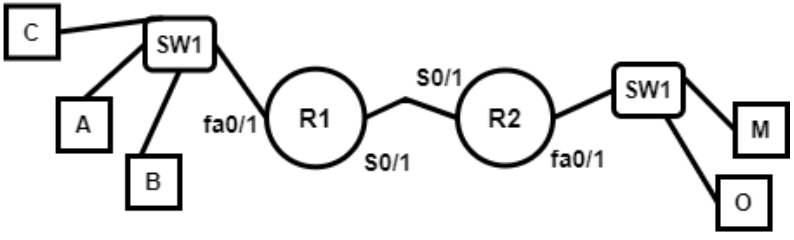
\includegraphics[width=0.7\textwidth]{p2_q6b_topology.png}
\end{center}

\textbf{Problem Statement:}
Host A wants to communicate with Host M. Host A knows the IP address of M. To complete the destination MAC address field, Host A performs an ARP.
\begin{enumerate}
    \item \textbf{Which device's IP address will Host A send the ARP for? [3 Marks]}
    \begin{itemize}
        \item Host A compares Host M's IP address with its own subnet mask and determines that Host M is located on a \textbf{different (remote) subnet}.
        \item Because Layer 2 frames cannot cross routers, Host A cannot send an ARP request directly for Host M.
        \item Instead, Host A must forward the packet to its \textbf{Default Gateway (Router R1's interface \texttt{fa0/1})}.
        \item Therefore, Host A sends the ARP request for the \textbf{IP address of Router R1's interface \texttt{fa0/1}}.
    \end{itemize}
    \item \textbf{After receiving the ARP reply, what will Host A do next? [4 Marks]}
    \begin{itemize}
        \item Host A caches Router R1's MAC address in its local ARP table.
        \item Host A encapsulates the IP datagram (with Source IP = Host A, Destination IP = Host M) into an Ethernet frame.
        \item Host A sets the frame header's \textbf{Destination MAC to Router R1's \texttt{fa0/1} MAC address} and Source MAC to Host A's MAC address.
        \item Host A transmits the Ethernet frame onto the local LAN towards switch SW1.
    \end{itemize}
\end{enumerate}

\vspace{0.2cm}
\textbf{6.c) [9 Marks] Switch MAC Table Learning \& Forwarding Analysis}

\begin{center}
    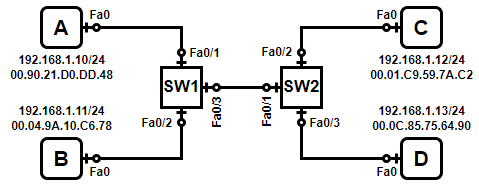
\includegraphics[width=0.65\textwidth]{p2_q6c_topology.png}
\end{center}

\textbf{Initial Conditions:}
\begin{itemize}
    \item SW1 contains: Host D (\texttt{00.0C.85.75.64.90}) on \texttt{Fa0/3}, Host A (\texttt{00.90.21.D0.DD.48}) on \texttt{Fa0/1}.
    \item SW2 is initially empty.
    \item Host B (\texttt{00.04.9A.10.C6.78}) on SW1 \texttt{Fa0/2} sends an ARP request for Host C's MAC address (\texttt{00.01.C9.59.7A.C2}) on SW2 \texttt{Fa0/2}.
\end{itemize}

\textbf{I. Step-by-Step Switch Actions (Flooding vs. Unicasting) [5 Marks]:}
\begin{enumerate}
    \item \textbf{ARP Request from Host B enters SW1 on \texttt{Fa0/2}:}
    \begin{itemize}
        \item Source MAC = \texttt{00.04.9A.10.C6.78} (Host B), Destination MAC = \texttt{FF:FF:FF:FF:FF:FF} (Broadcast).
        \item \textbf{Learning:} SW1 records: MAC of Host B on port \texttt{Fa0/2}.
        \item \textbf{Forwarding:} Because destination is broadcast, SW1 \textbf{floods} the frame out of all other ports: \texttt{Fa0/1} (to Host A) and \texttt{Fa0/3} (to SW2).
    \end{itemize}

    \item \textbf{ARP Request enters SW2 on \texttt{Fa0/1}:}
    \begin{itemize}
        \item \textbf{Learning:} SW2 records: MAC of Host B on port \texttt{Fa0/1}.
        \item \textbf{Forwarding:} Since destination is broadcast, SW2 \textbf{floods} the frame out of all other ports: \texttt{Fa0/2} (to Host C) and \texttt{Fa0/3} (to Host D).
    \end{itemize}

    \item \textbf{Host C generates unicast ARP Reply:}
    \begin{itemize}
        \item Source MAC = Host C (\texttt{00.01.C9.59.7A.C2}), Destination MAC = Host B (\texttt{00.04.9A.10.C6.78}).
        \item Frame enters SW2 on port \texttt{Fa0/2}.
        \item \textbf{Learning on SW2:} SW2 learns: MAC of Host C on port \texttt{Fa0/2}.
        \item \textbf{Forwarding on SW2:} SW2 looks up destination MAC (Host B). SW2 already has Host B on port \texttt{Fa0/1}! Therefore, SW2 \textbf{unicasts} the reply directly and solely out of port \texttt{Fa0/1} towards SW1 (it does \emph{not} flood to Host D).
    \end{itemize}

    \item \textbf{ARP Reply enters SW1 on port \texttt{Fa0/3}:}
    \begin{itemize}
        \item \textbf{Learning on SW1:} SW1 learns: MAC of Host C on port \texttt{Fa0/3}.
        \item \textbf{Forwarding on SW1:} SW1 looks up destination MAC (Host B), finds it in its table on \texttt{Fa0/2}, and \textbf{unicasts} the frame directly out of port \texttt{Fa0/2} to Host B.
    \end{itemize}
\end{enumerate}

\textbf{II. Updated MAC Address Tables of Both Switches [4 Marks]:}

\begin{center}
\begin{tabular}{|l|c|}
\multicolumn{2}{c}{\textbf{Switch SW1 MAC Table}} \\
\hline
\textbf{MAC Address} & \textbf{Port} \\
\hline
\texttt{00.90.21.D0.DD.48} (Host A) & \texttt{Fa0/1} \\
\texttt{00.04.9A.10.C6.78} (Host B) & \texttt{Fa0/2} \\
\texttt{00.0C.85.75.64.90} (Host D) & \texttt{Fa0/3} \\
\texttt{00.01.C9.59.7A.C2} (Host C) & \texttt{Fa0/3} \\
\hline
\end{tabular}
\qquad
\begin{tabular}{|l|c|}
\multicolumn{2}{c}{\textbf{Switch SW2 MAC Table}} \\
\hline
\textbf{MAC Address} & \textbf{Port} \\
\hline
\texttt{00.04.9A.10.C6.78} (Host B) & \texttt{Fa0/1} \\
\texttt{00.01.C9.59.7A.C2} (Host C) & \texttt{Fa0/2} \\
\hline
\end{tabular}
\end{center}

\begin{center}
    \rule{\textwidth}{0.8pt}\\[3pt]
    \textbf{\textcolor{primary}{--- END OF EXAMINATION SOLUTION ---}}
\end{center}

\end{document}
